\documentclass{article}

\usepackage[top=3cm, bottom=3cm, left=3cm, right=3cm]{geometry}

\usepackage[utf8]{inputenc}
\usepackage[T1]{fontenc}
\usepackage[frenchb]{babel}

\usepackage[a4paper,colorlinks,linkcolor=darkgray,citecolor=red,urlcolor=blue]{hyperref}
\usepackage{graphicx}
\usepackage{caption}
\usepackage{subcaption}
\usepackage{amsthm}
\usepackage{listings}
\usepackage{tikz}
\usepackage{algorithm}
\usepackage{amsmath}
\usepackage[noend]{algpseudocode}
\usepackage{amsfonts}
\usepackage{amssymb}
\usepackage{authblk}

\usepackage{tikz} % Let us start the fun
\usetikzlibrary{positioning, chains, calc, arrows, decorations.pathreplacing, fit, patterns, snakes}

\theoremstyle{definition} 
\newtheorem{definition}{Définition} 

\makeatletter
 
\newskip\@bigflushglue \@bigflushglue = -100pt plus 1fil
 
\def\bigcenter{\trivlist \bigcentering\item\relax}
\def\bigcentering{\let\\\@centercr\rightskip\@bigflushglue%
\leftskip\@bigflushglue
\parindent\z@\parfillskip\z@skip}
\def\endbigcenter{\endtrivlist}
 
\makeatother

\renewcommand\Affilfont{\small}

\title{Projet Images}

\author[$\dag$]{Laureline Pinault et Raphaël Charrondière}
\affil[$\dag$]{ENS de Lyon, France}

\date{Lundi 4 mai 2015}

\begin{document}

  \maketitle

  \begin{abstract}
	Laureline Pinault et Raphaël Charrondière sont fiers de vous présenter leur classificateur d'images !
  \end{abstract}
  
  \newpage

  \tableofcontents

  \newpage
  
  \section{Introduction}

    \subsection{Objectifs du projet}
    	Ce projet a pour but de coder un classificateur d'images en noir et blanc. Un classificateur d'images est un programme qui étant donné une image en entrée renvoie sa classe. Une classe représente un objet. Par exemple une image peut appartenir à la classe pomme si elle représente une pomme.

    \subsection{Remarques préliminaires}    	
    	Ce projet est réalisé en c++  et s'appuie sur la bibliothèque DGtal.
    	  
  \section{Organisation du projet} %TODO : Raphaël
  	Ce projet a été réalisé de manière très modulaire. Il ne s'agit pas d'un classificateur unique, mais de petits classificateurs qui combinés deviennent à priori plus précis. Ainsi le choix a été fait de créer des bibliothèques chargées dynamiquement par le programme central qui les exécute les uns après les autres. L'avantage de procéder ainsi est de cloisonner chaque classificateur (que l'on appellera aussi estimateur) afin qu'aucun n'infère sur l'autre. En particulier si l'un dysfonctionne il ne perturbe pas le déroulement du programme ou il suffit juste le supprimer.
  	   
  	   \subsection{Estimateur, comment ça fonctionne}
	Un classificateur ne renvoie pas directement une classe, en fait il va comparer un modèle à une image et dire selon lui comment le modèle et l'image sont éloignés. Du point de vue extérieur un estimateur comporte trois fonctions : \verb-buildmodel-, \verb-pre_estim- et \verb-estim-. La première donne une liste de fichier d'une même classe et renvoie un modèle, celui-ce pouvant être quelconque (un entier ou un graphe par exemple). La deuxième demande de réduire l'image à une donnée, la motivation étant de pouvoir rapidement comparer cette donnée à plusieurs modèles, cette comparaison étant faite par la troisième fonction.
  
  
  \section{Traitement des images}
  
  	Il est à noter que les traitements sur images ne sont pas systématiquement appliqués. Chaque estimateur peut l'appliquer s'il en a besoin, selon la résistance au bruit, à l'agrandissement d'image, etc.
  
    \subsection{Traitement anti-inversion}
    
      \begin{figure}[!h]
	\centering
	\begin{subfigure}{.49\textwidth}
	  \begin{subfigure}{.49\textwidth}
	    \centering
	    \includegraphics[scale=0.25]{Illustrations/rat-8.png}
	    \label{1strat}
	  \end{subfigure}
	  \begin{subfigure}{.49\textwidth}
	    \centering
	    \includegraphics[scale=0.25]{Illustrations/rat-8-inverse.png}
	    \label{1strat-inverse}
	  \end{subfigure}
	  \subcaption{Ce rat n'a pas été inversé}
	\end{subfigure}
	\begin{subfigure}{.49\textwidth}
	  \begin{subfigure}{.49\textwidth}
	    \centering
	    \includegraphics[scale=0.25]{Illustrations/rat-9.png}
	  \label{2ndrat}
	  \end{subfigure}
	  \begin{subfigure}{.49\textwidth}
	    \centering
	    \includegraphics[scale=0.25]{Illustrations/rat-9-inverse.png}
	  \label{2ndrat-inverse}
	  \end{subfigure}
	  \subcaption{Ce rat a été inversé}
	\end{subfigure}
	\caption{Inversion de l'objet rat}
	\label{anti-inversion}
      \end{figure}

    \subsection{Normalisation des images}     %TODO : Raphaël
    
    Cette opération consiste d'abord à calculer le centre de gravité $G$ de l'objet, puis à calculer l'éloignement moyen $m$ à celui-ci, c'est à dire le distance moyenne point de l'objet à son centre de gravité.
    
    Ensuite, on crée un nouvelle image d'une taille $800 \times 800$ correspondant à l'image recentrée en G affichant les points d'origines de la fenêtre de taille $4m \times 4m$.
    
    Cela permet d'avoir un objet normé en taille et centré (donc est idéal pour des estimateurs travaillant sur l'aire ou sensible aux translations).
      
    \subsection{Traitement anti-bruit}
    
    \subsection{Remplissage}
    \label{sec:remplissage}
    
      \begin{figure}[!h]
	\centering
	\begin{subfigure}{.25\textwidth}
	  \centering
	  \includegraphics[scale=0.30]{Illustrations/pocket-20.png}
	  \label{pocket-non-rempli}
	\end{subfigure}
	\begin{subfigure}{.25\textwidth}
	  \centering
	  \includegraphics[scale=0.30]{Illustrations/pocket-20-rempli.png}
	\label{pocket-rempli}
	\end{subfigure}
	\caption{Remplissage de l'objet pocket}
	\label{remplissage}
      \end{figure}
      
      \begin{figure}[!h]
	\centering
	\begin{subfigure}{.47\textwidth}
	  \begin{subfigure}{.52\textwidth}
	    \centering
	    \includegraphics[scale=0.295]{Illustrations/butterfly-10-rempli.png}
	    \label{butterfly-rempli}
	  \end{subfigure}
	  \begin{subfigure}{.45\textwidth}
	    \centering
	    \includegraphics[scale=0.16]{Illustrations/device9-6-rempli.png}
	    \label{spirale-rempli}
	  \end{subfigure}
	  \subcaption{Certains détails ne sont pas remplis}
	\end{subfigure}
	\begin{subfigure}{.44\textwidth}
	  \begin{subfigure}{.46\textwidth}
	    \centering
	    \includegraphics[scale=0.25]{Illustrations/cup-7-rempli.png}
	  \label{1stcup-rempli}
	  \end{subfigure}
	  \begin{subfigure}{.46\textwidth}
	    \centering
	    \includegraphics[scale=0.275]{Illustrations/cup-12-rempli.png}
	  \label{2ndcup-rempli}
	  \end{subfigure}
	  \subcaption{Les tasses ne sont pas remplies pareil}
	\end{subfigure}
	\caption{Problèmes soulevés par le remplissage des objets}
	\label{problèmes-remplissage}
      \end{figure}      
   
  \section{Estimateurs}
  
    \subsection{Quelques estimateurs simples et complémentaires}

      Une première idée fut de travailler sur la forme générale de la forme \textendash est-ce qu'elle est plutôt carré ? ronde ? allongée ? Pour cela, trois estimateurs simples et complémentaires ont été développés. Tous tentent de décrire une image par un simple scalaire.
      
      L'estimateur \texttt{estimeccentricity} qui mesure l'excentricité d'une forme permet de déterminer si la forme est plus ou moins allongée. L'estimateur \texttt{estimaveragebendingflexion}, qui n'est pas opérationnel suite à des erreurs de programmation\footnote{Il sera néanmoins présenté dans ce rapport}, devait mesurer l'énergie moyenne de flexion afin de pouvoir distinguer les formes arrondies, très arrondies ou plates. Enfin l'estimateur \texttt{estimsolidity} qui mesure la solidité d'une forme apporte une information sur comment la forme remplit son enveloppe convexe. %fin à retravailler
    
      \subsubsection{Solidité}
      
	\paragraph{Principe}
	
	  \begin{definition}[Solidité]
	    On définit la solidité d'une forme comme le rapport de l'aire de cette forme sur l'aire de l'enveloppe convexe.
	  \end{definition}

	   Une illustration de ce que représente la solidité est donnée Figure \ref{solidité}.
	
	  \begin{figure}[!h]
	    \centering
	    \begin{subfigure}{.25\textwidth}
	      \centering
	      \includegraphics[scale=0.30]{Illustrations/horse-20.png}
	      \label{horse}
	    \end{subfigure}
	    \begin{subfigure}{.25\textwidth}
	      \centering
	      \includegraphics[scale=0.30]{Illustrations/horse-20-rempli-convexhull.png}
	    \label{horse-rempli-convexhull}
	    \end{subfigure}
	    \caption{Solidité de l'objet horse}
	    \label{solidité}
	  \end{figure}
	
	\paragraph{Programmation}
	
	  Pour calculer la solidité d'une form, on procède de la façon suivante :
	  \begin{itemize}
	   \item Afin de ne pas être pas être trop dépendant de la qualité de l'image donné en entré, on commence par éliminer les détails interne en effectuant un remplissage de la forme (voir Section \ref{sec:remplissage}).
	   \item On calcule ensuite l'aire de la forme ainsi obtenue. Pour calculer l'aire d'une forme, on procède tout simplement à un comptage du nombre de pixels blancs. Cette manière de procéder a le double avantage d'être simple à implémenter et d'être convergente, ce qui permettra de ne pas être dépendant de l'échelle de l'image.
	   \item On détermine ensuite les points de l'image faisant partie de l'enveloppe convexe de la forme grâce .
	  \end{itemize}
  
	
	\paragraph{Résistance aux inversions de couleur}
	
	\paragraph{Résistance au bruit}
	
%	pour résumer :
%- quand le bruit devient vraiment important (genre 0.8), ça a tendance a foirer que ce soit debruité ou pas
%- sinon c'est plutot pas mal
%- par contre l'estimateur avec et sans débruitage sont assez loin
%=> il faut le modèle avec un traitement anti bruit

	
	\paragraph{Résistance aux rotations et symmétries}
      
	\paragraph{Résistance aux homothéties} blabla \\
	
	  \begin{table}[!h]
	  \centering
	  \begin{tabular}{|c|c|c|c|c|c|c|c|}
	    \hline
	    \multicolumn{2}{|c|}{Cheval} & \multicolumn{2}{|c|}{Pomme} & \multicolumn{2}{|c|}{Device} & \multicolumn{2}{|c|}{Lézard} \\
	    \multicolumn{2}{|c|}{\includegraphics[scale=0.15]{Illustrations/horse-20.png}} 
	    & \multicolumn{2}{|c|}{\includegraphics[scale=0.15]{Illustrations/apple-3.png}} 
	    & \multicolumn{2}{|c|}{\includegraphics[scale=0.075]{Illustrations/device7-1.png}} 
	    & \multicolumn{2}{|c|}{\includegraphics[scale=0.09]{Illustrations/lizzard-13.png}} \\
	    \hline
	    \textbf{Echelle} & \textbf{Solidité} & \textbf{Echelle} & \textbf{Solidité} & \textbf{Echelle} & \textbf{Solidité} & \textbf{Echelle} & \textbf{Solidité} \\
	    \hline
	    0.5 & 0.584583 & 0.5 & 0.933504 & 0.5 & 0.77016 & 0.5 & 0.767554 \\
	    \hline
	    1 & 0.577491 & 1 & 0.931911 & 1 & 0.768281 & 1 & 0.762166 \\
	    \hline
	    2 & 0.57244 & 2 & 0.930546 & 2 & 0.767288 & 2 & 0.75678 \\
	    \hline
	    5 & 0.569273 & 5 & 0.929267 & 5 & 0.703692 & 5 & 0.7533 \\
	    \hline
	  \end{tabular}
	  \caption{Variations de la solidité de plusieurs objets selon l'agrandissement}
	  \label{solidité-scaling-table}
	  \end{table}
	  
	\paragraph{Résistance aux élongations}
	
	\paragraph{Résistance aux occlusions}
	  
	\paragraph{Résultats}
	
	  \begin{figure}[!h]
	    \begin{bigcenter}
	      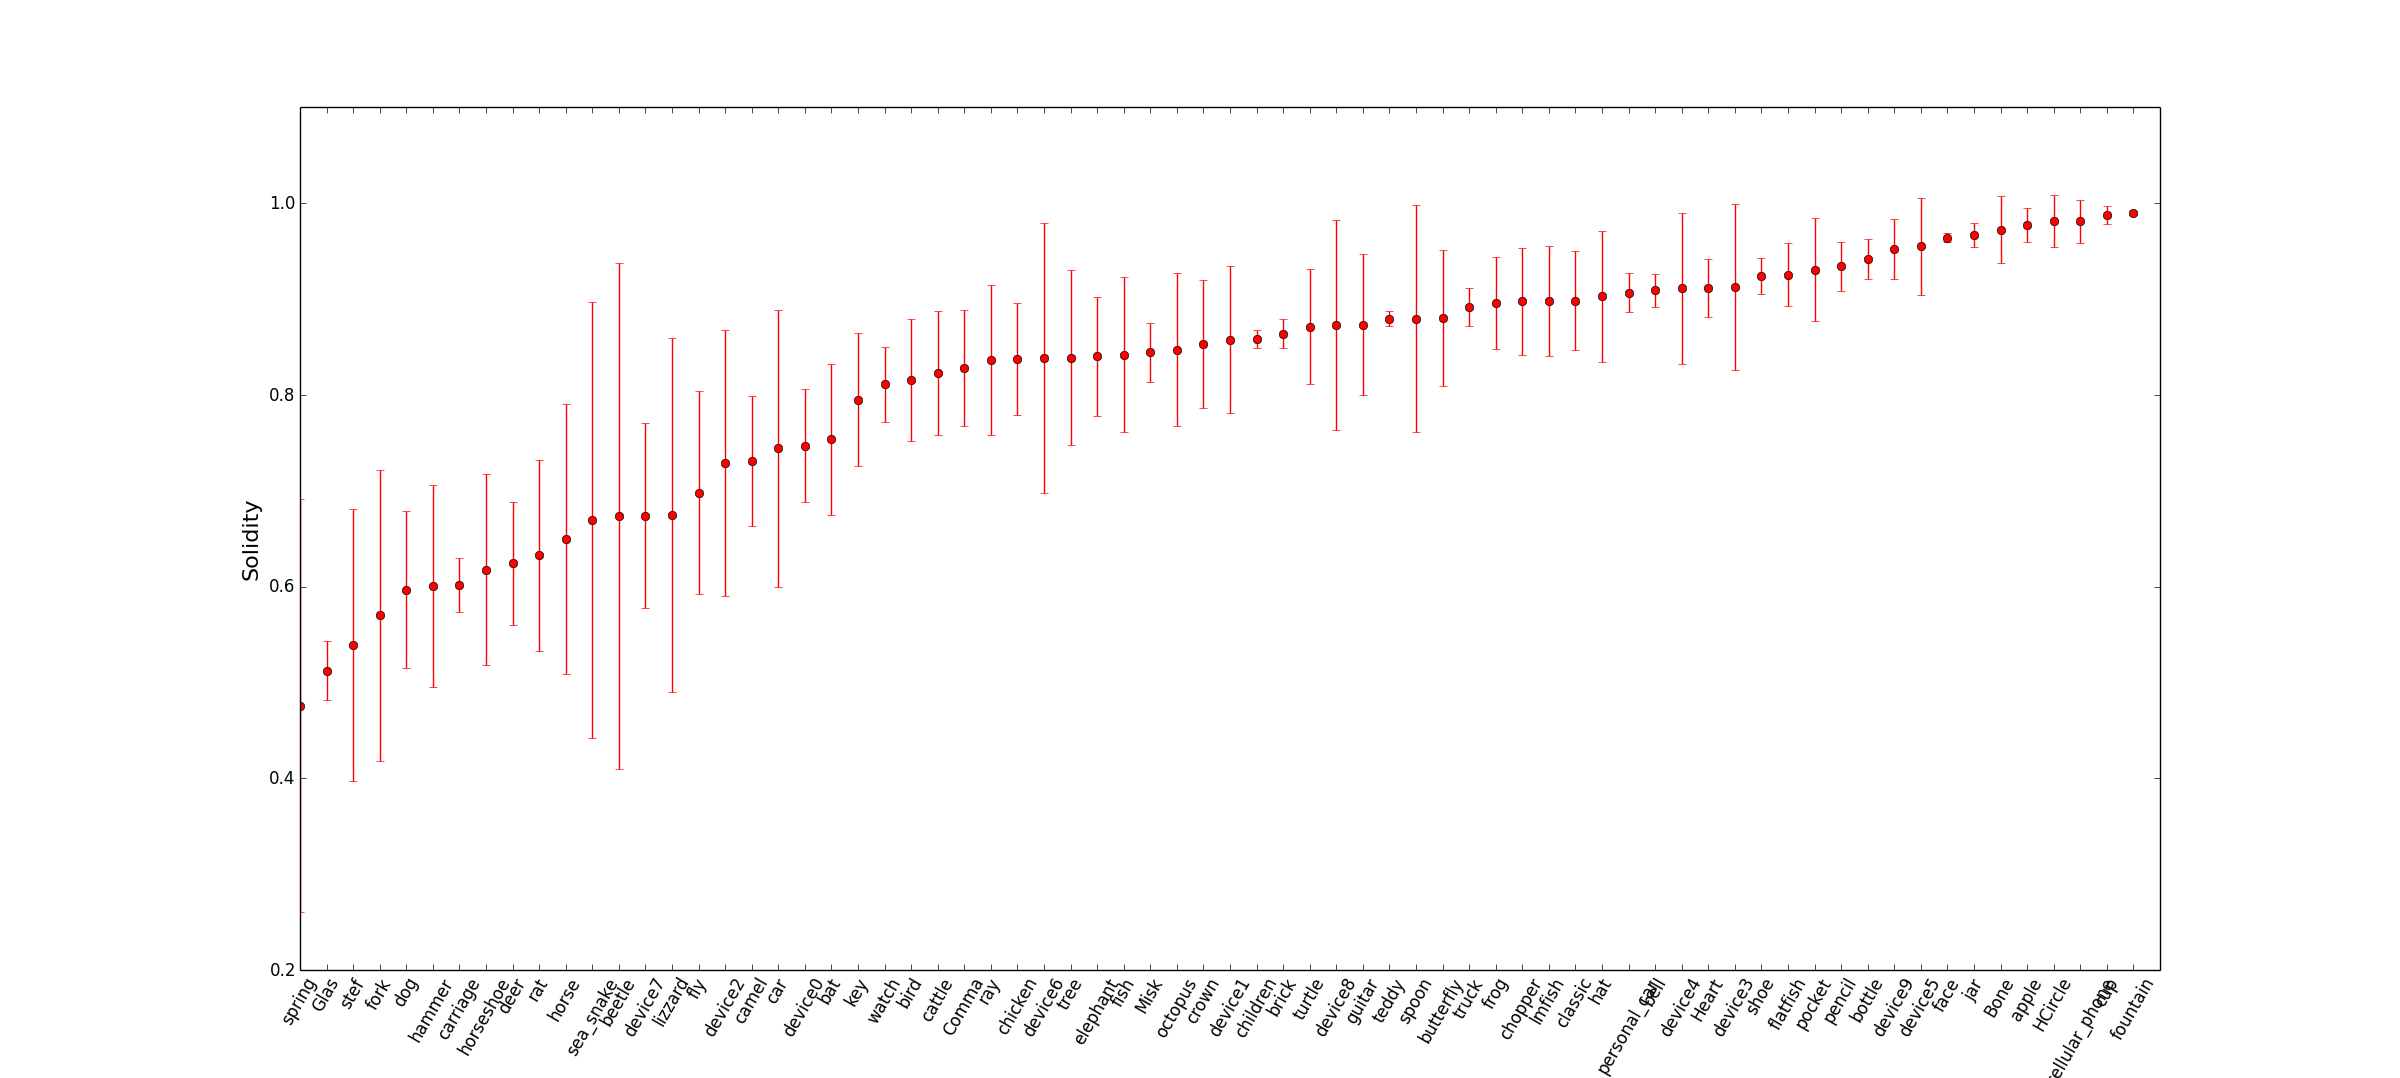
\includegraphics[scale=0.38]{Graphes/solidite.png}
	    \end{bigcenter}
	    \caption{Moyenne et écart type de la solidité pour chaque classe}
	    \label{solidité-graph}
	  \end{figure}

      \subsubsection{Excentricté}
      
	\paragraph{Principe}
      
	\paragraph{Programmation}
	
	\paragraph{Résistance aux inversions de couleur}
	
	\paragraph{Résistance au bruit}
	
	\paragraph{Résistance aux rotations et symmétries}
      
	\paragraph{Résistance aux homothéties} blabla
	
	
	  \begin{table}[!h]
	  \centering      
	  \begin{tabular}{|c|c|c|c|c|c|}
	    \hline
	    \multicolumn{2}{|c|}{Chauve-souris} & \multicolumn{2}{|c|}{Marteau} & \multicolumn{2}{|c|}{Device}  \\
	    \multicolumn{2}{|c|}{
\includegraphics[scale=0.11]{Illustrations/bat-2.png}} 
	    & \multicolumn{2}{|c|}{
\includegraphics[scale=0.15]{Illustrations/hammer-20.png}} 
	    & \multicolumn{2}{|c|}{
\includegraphics[scale=0.07]{Illustrations/device9-9.png}}  \\
	    \hline
	    \textbf{Echelle} & \textbf{Excentricité} & \textbf{Echelle} & \textbf{Excentricité} & \textbf{Echelle} & \textbf{Excentricité} \\
	    \hline
	    0.5 & 2.32927 & 0.5 & 2.92308 & 0.5 & 1.0101 \\
	    \hline
	    1 & 2.33841 & 1 & 2.89873 & 1 & 1.01515 \\
	    \hline
	    2 & 2.33994 & 2 & 2.91772 & 2 & 1.01641 \\
	    \hline
	    5 & 2.34065 & 5 & 2.92152 & 5 & 1.01767 \\
	    \hline
	  \end{tabular}
	  \caption{Variations de l'excentricité de plusieurs objets selon l'agrandissement}
	  \label{excentricité-scaling-table}
	  \end{table}  
	  
	\paragraph{Résistance aux élongations}
	
	\paragraph{Résistance aux occlusions}
	  
	\paragraph{Résultats}
	  

      
      \subsubsection{Energie de flexion moyenne}
      
	\paragraph{Principe}
	
	\paragraph{Programmation}
	
	  Méthode du cercle circonscrit par les deux demis tangentes.
	  
	  \begin{figure}[!h]
	    \centering
	    \begin{tikzpicture}
	    \begin{scope}[scale = .4]
	      \draw (0,0) circle (5);
	      \node[] at (30:5) (Q) {\textbullet};
	      \node[right=.01cm of Q] {$Q$};
	      \node[] at (80:5) (P) {\textbullet};
	      \node[above=.01cm of P] {$P$};
	      \node[] at (165:5) (O) {\textbullet};
	      \node[left=.01cm of O] {$O$};
	      \draw[] (30:5) -- (80:5) -- (165:5) -- (30:5);
	      \node[] (C) {$\times$};
	      \node[below right=.01cm and .01cm of C] {$C$};
	      \draw[dashed] (0,0) -- node[right]{$r$} (80:5);
	    \end{scope}
	    \end{tikzpicture}
	    \caption{Cercle circonscrit au triangle OPQ}
	    \label{cercle-circonscrit}
	  \end{figure}
	  
	  Par la loi des sinus, $r = \frac{|QO|}{2 \sin\left(\widehat{OPQ}\right)}$. On en déduit que :
	  
	  \[ r = \frac{|QO|}{2 \sin\left(\widehat{OPQ}\right)} = \frac{|QO|}{\frac{2 \det\left(\overrightarrow{PO}, \overrightarrow{PQ} \right)}{|OP| |PQ|}} = \frac{|OP| |PQ| |QO|}{4 \mathcal{A}_{PQO}}  \]
	
	\paragraph{Résultats}
    
    \subsection{Transformée de Fourier}  %A mettre ? RAphaël
    
    \subsection{Méthode des moments} %A renommer ? Raphaël
    
    \subsection{Etude du squelette} %TODO : Raphaël
    
    \subsection{Pistes non explorées}
  
  \section{Résultats} 
  
    \subsection{Méthodologie d'estimation}  %En gros : c'est quoi nos résultats ?, je sais pas trop comment le nommer
    
    \subsection{Résultats} %Beaucoup de section / subsection = résultats
  
  \section{Conclusion}
  
\end{document}

